\documentclass[border=5pt]{standalone}
\usepackage[T1]{fontenc}
\usepackage{lmodern,amsmath,amssymb,tikz}
\usetikzlibrary{arrows.meta,calc,fit,backgrounds}
\renewcommand{\familydefault}{\sfdefault}
\definecolor{edge}{HTML}{36424B}
\definecolor{spatial}{HTML}{E0EFEB}
\definecolor{temporal}{HTML}{E8E5F3}
\definecolor{stem}{HTML}{E5EDF7}
\definecolor{latent}{HTML}{F8EDDA}
\begin{document}
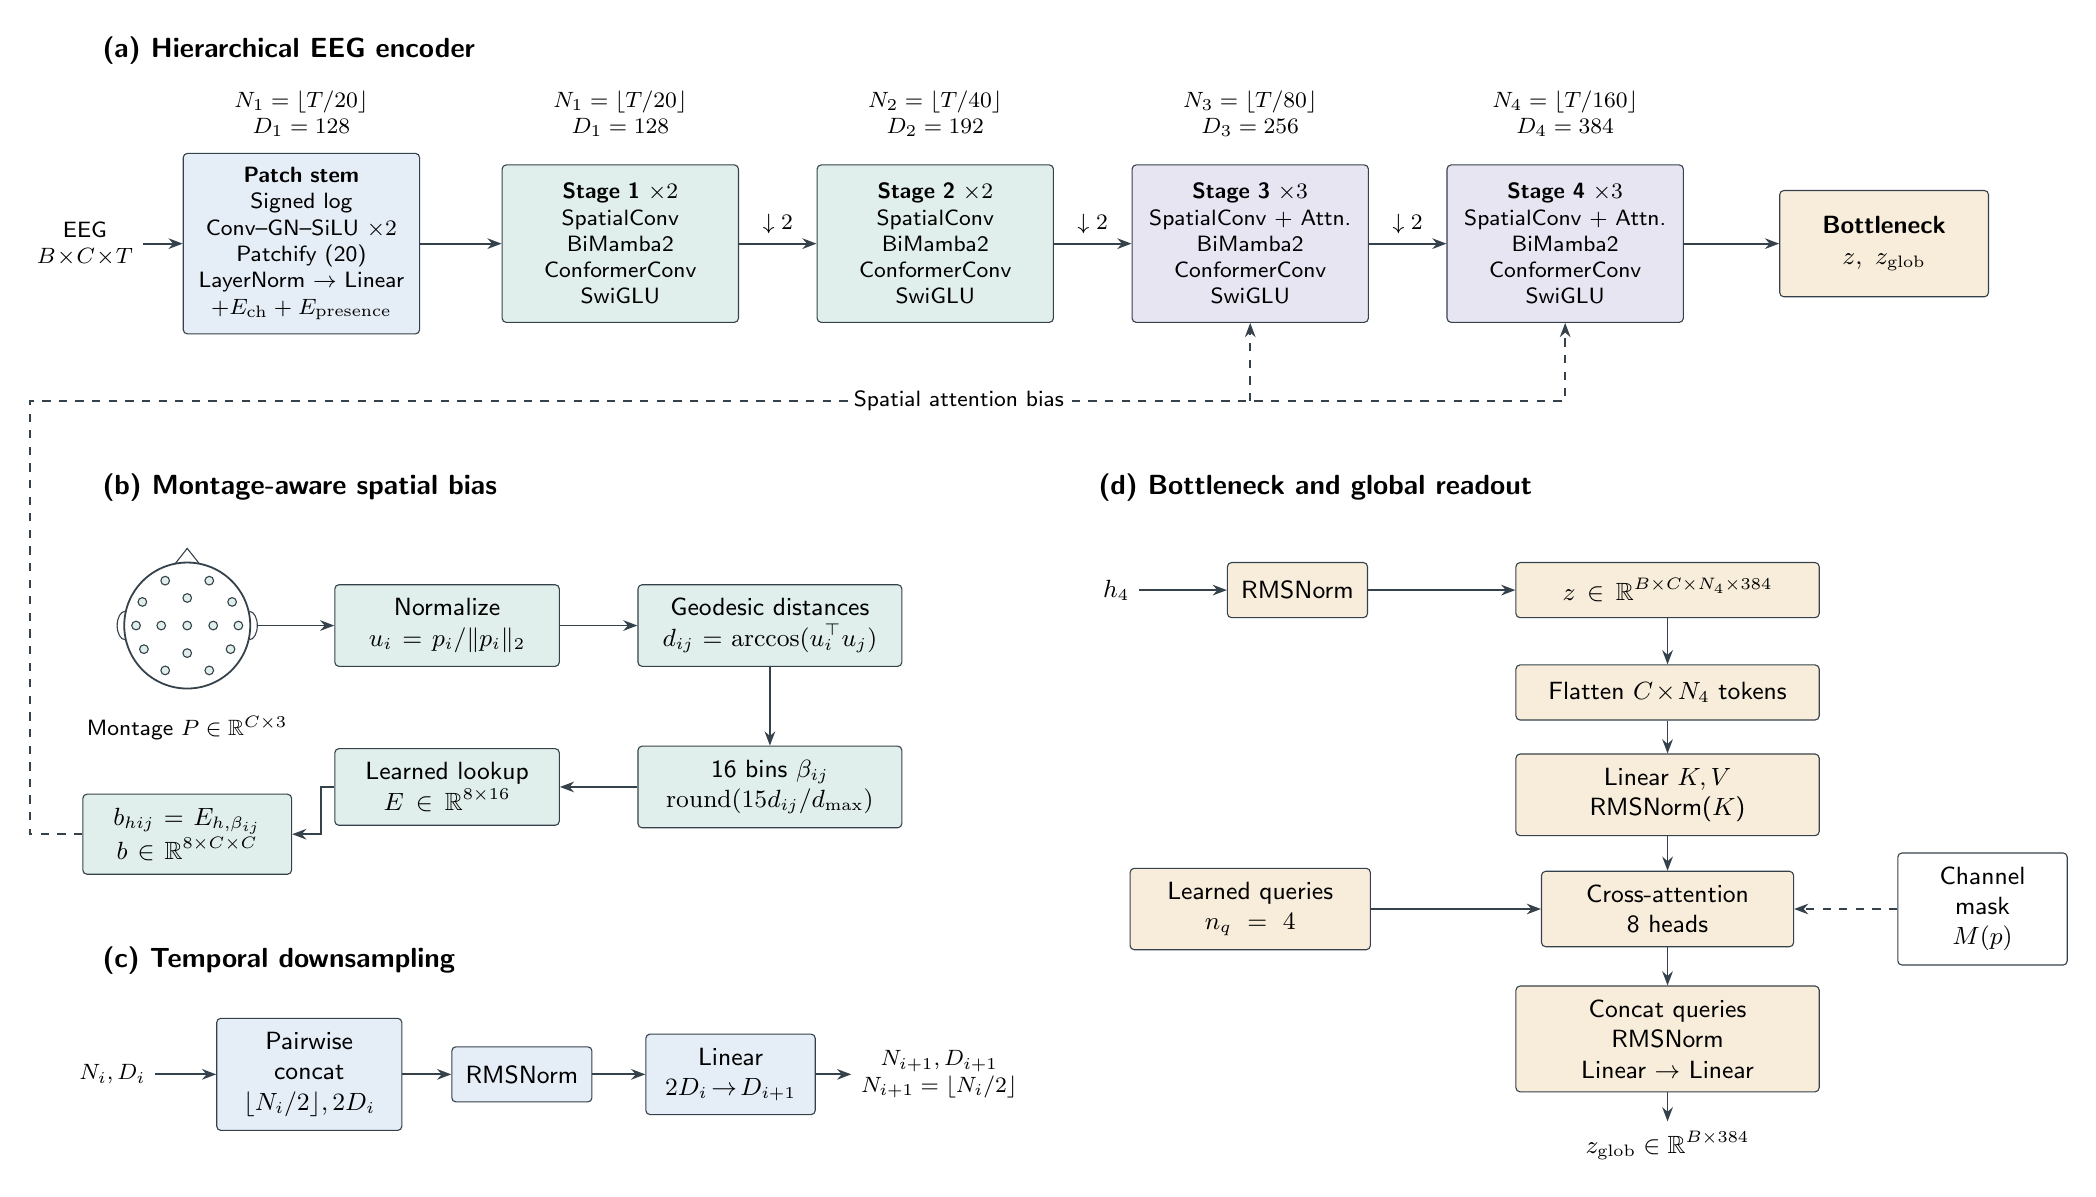
\begin{tikzpicture}[font=\small,x=1cm,y=1cm,>={Stealth[length=1.8mm]},
 block/.style={draw=edge,rounded corners=1.5pt,align=center,inner sep=5pt,minimum height=.7cm},
 stage/.style={block,text width=2.65cm,font=\footnotesize,minimum height=2cm},
 flow/.style={->,draw=edge,line width=.65pt},
 cond/.style={flow,dashed},
 panel/.style={font=\bfseries,anchor=west},
 label/.style={font=\footnotesize,align=center}]
\node[panel] at (0,2.45) {(a) Hierarchical EEG encoder};
\node[label] (x) at (-.1,0) {EEG\\$B\!\times\!C\!\times\!T$};
\node[stage,fill=stem] (stem) at (2.65,0) {\textbf{Patch stem}\\Signed log\\Conv--GN--SiLU $\times2$\\Patchify (20)\\LayerNorm $\to$ Linear\\$+E_{\rm ch}+E_{\rm presence}$};
\node[stage,fill=spatial] (s1) at (6.7,0) {\textbf{Stage 1 $\times2$}\\SpatialConv\\BiMamba2\\ConformerConv\\SwiGLU};
\node[stage,fill=spatial] (s2) at (10.7,0) {\textbf{Stage 2 $\times2$}\\SpatialConv\\BiMamba2\\ConformerConv\\SwiGLU};
\node[stage,fill=temporal] (s3) at (14.7,0) {\textbf{Stage 3 $\times3$}\\SpatialConv + Attn.\\BiMamba2\\ConformerConv\\SwiGLU};
\node[stage,fill=temporal] (s4) at (18.7,0) {\textbf{Stage 4 $\times3$}\\SpatialConv + Attn.\\BiMamba2\\ConformerConv\\SwiGLU};
\node[block,fill=latent,text width=2.3cm,minimum height=1.35cm] (bott) at (22.75,0) {\textbf{Bottleneck}\\$z,\ z_{\rm glob}$};
\draw[flow] (x)--(stem); \draw[flow] (stem)--(s1);
\draw[flow] (s1)--node[above,label]{$\downarrow2$}(s2);
\draw[flow] (s2)--node[above,label]{$\downarrow2$}(s3);
\draw[flow] (s3)--node[above,label]{$\downarrow2$}(s4);
\draw[flow] (s4)--(bott);
\node[label] at (2.65,1.65) {$N_1=\lfloor T/20\rfloor$\\$D_1=128$};
\node[label] at (6.7,1.65) {$N_1=\lfloor T/20\rfloor$\\$D_1=128$};
\node[label] at (10.7,1.65) {$N_2=\lfloor T/40\rfloor$\\$D_2=192$};
\node[label] at (14.7,1.65) {$N_3=\lfloor T/80\rfloor$\\$D_3=256$};
\node[label] at (18.7,1.65) {$N_4=\lfloor T/160\rfloor$\\$D_4=384$};

\node[panel] at (0,-3.1) {(b) Montage-aware spatial bias};
% Schematic electrode montage (positions supplied by standard_1020).
\begin{scope}[shift={(1.2,-4.85)}]
\draw[edge,line width=.65pt] (0,0) circle (.8);
\draw[edge] (-.15,.79)--(0,.98)--(.15,.79);
\draw[edge] (-.79,.18) arc[start angle=90,end angle=270,x radius=.1,y radius=.18];
\draw[edge] (.79,.18) arc[start angle=90,end angle=-90,x radius=.1,y radius=.18];
\foreach \xx/\yy in {-.28/.57,.28/.57,-.57/.3,0/.35,.57/.3,-.65/0,-.33/0,0/0,.33/0,.65/0,-.55/-.3,0/-.35,.55/-.3,-.28/-.57,.28/-.57}{
\filldraw[draw=edge,fill=spatial] (\xx,\yy) circle (.055);
}
\end{scope}
\node[label] at (1.2,-6.15) {Montage $P\in\mathbb{R}^{C\times3}$};
\node[block,fill=spatial,text width=2.5cm] (unit) at (4.5,-4.85) {Normalize\\$u_i=p_i/\|p_i\|_2$};
\node[block,fill=spatial,text width=3cm] (geo) at (8.6,-4.85) {Geodesic distances\\$d_{ij}=\arccos(u_i^\top u_j)$};
\node[block,fill=spatial,text width=3cm] (bins) at (8.6,-6.9) {16 bins $\beta_{ij}$\\$\operatorname{round}(15d_{ij}/d_{\max})$};
\node[block,fill=spatial,text width=2.5cm] (lookup) at (4.5,-6.9) {Learned lookup\\$E\in\mathbb{R}^{8\times16}$};
\node[block,fill=spatial,text width=2.3cm] (bias) at (1.2,-7.5) {$b_{hij}=E_{h,\beta_{ij}}$\\$b\in\mathbb{R}^{8\times C\times C}$};
\draw[flow] (2.1,-4.85)--(unit); \draw[flow] (unit)--(geo);
\draw[flow] (geo)--(bins); \draw[flow] (bins)--(lookup);
\draw[flow] (lookup.west)--(2.9,-6.9)|-(bias.east);
\draw[cond] (bias.west)--(-.8,-7.5)--(-.8,-2)--(18.7,-2)--(s4.south);
\draw[cond] (14.7,-2)--(s3.south);
\node[label,fill=white,inner sep=2pt] at (11,-2) {Spatial attention bias};

\node[panel] at (0,-9.1) {(c) Temporal downsampling};
\node[label] (di) at (.25,-10.55) {$N_i,D_i$};
\node[block,fill=stem,text width=2cm] (pair) at (2.75,-10.55) {Pairwise concat\\$\lfloor N_i/2\rfloor,2D_i$};
\node[block,fill=stem] (dn) at (5.45,-10.55) {RMSNorm};
\node[block,fill=stem,text width=1.8cm] (dp) at (8.1,-10.55) {Linear\\$2D_i\!\to\!D_{i+1}$};
\node[label] (do) at (10.75,-10.55) {$N_{i+1},D_{i+1}$\\$N_{i+1}=\lfloor N_i/2\rfloor$};
\draw[flow] (di)--(pair); \draw[flow] (pair)--(dn); \draw[flow] (dn)--(dp); \draw[flow] (dp)--(do);

\node[panel] at (12.65,-3.1) {(d) Bottleneck and global readout};
\node (h) at (13,-4.4) {$h_4$};
\node[block,fill=latent] (bn) at (15.3,-4.4) {RMSNorm};
\node[block,fill=latent,text width=3.5cm] (z) at (20,-4.4) {$z\in\mathbb{R}^{B\times C\times N_4\times384}$};
\node[block,fill=latent,text width=3.5cm] (flat) at (20,-5.7) {Flatten $C\!\times\!N_4$ tokens};
\node[block,fill=latent,text width=3.5cm] (kv) at (20,-7) {Linear $K,V$\\RMSNorm($K$)};
\node[block,fill=latent,text width=2.85cm] (attn) at (20,-8.45) {Cross-attention\\8 heads};
\node[block,fill=latent,text width=2.7cm] (query) at (14.7,-8.45) {Learned queries\\$n_q=4$};
\node[block,text width=1.8cm] (mask) at (24,-8.45) {Channel mask\\$M(p)$};
\node[block,fill=latent,text width=3.5cm] (merge) at (20,-10.1) {Concat queries\\RMSNorm\\Linear $\to$ Linear};
\node (global) at (20,-11.45) {$z_{\rm glob}\in\mathbb{R}^{B\times384}$};
\draw[flow] (h)--(bn); \draw[flow] (bn)--(z); \draw[flow] (z)--(flat);
\draw[flow] (flat)--(kv); \draw[flow] (kv)--(attn);
\draw[flow] (query)--(attn); \draw[cond] (mask)--(attn);
\draw[flow] (attn)--(merge); \draw[flow] (merge)--(global);
\end{tikzpicture}
\end{document}
